\documentclass[crop,border=0pt]{standalone}

\usepackage{mathtools}
\usepackage{tikz}
\usetikzlibrary{fit,positioning,scopes,arrows,decorations.pathreplacing}

\begin{document}
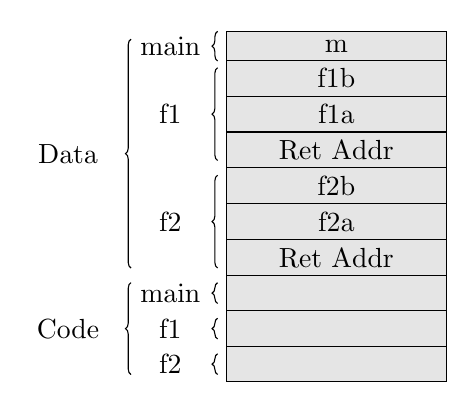
\begin{tikzpicture}[
  mybox/.style={
    fill=gray!20, minimum width=2.8cm, minimum height=1em, inner sep=3pt, draw
  },
  mydec/.style={
    decorate,decoration={brace,amplitude=2pt}
  },
  node distance=-\pgflinewidth]

  \node [mybox] (m) {m};
  \draw [mydec] ([xshift=-.1cm]m.south west) -- ([xshift=-.1cm]m.north west) node [black,midway,xshift=-0.6cm] {main};

  \node [mybox, below=of m] (f1b) {f1b};
  \node [mybox, below=of f1b] (f1a) {f1a};
  \node [mybox, below=of f1a] (f1r) {Ret Addr};
  \draw [mydec] ([xshift=-.1cm,yshift=1mm]f1r.south west) -- ([xshift=-.1cm,yshift=-1mm]f1b.north west) node [black,midway,xshift=-0.6cm] {f1};

  \node [mybox, below=of f1r] (f2b) {f2b};
  \node [mybox, below=of f2b] (f2a) {f2a};
  \node [mybox, below=of f2a] (f2r) {Ret Addr};
  \draw [mydec] ([xshift=-.1cm,yshift=1mm]f2r.south west) -- ([xshift=-.1cm,yshift=-1mm]f2b.north west) node [black,midway,xshift=-0.6cm] {f2};

  \draw [mydec] ([xshift=-1.2cm,yshift=1mm]f2r.south west) -- ([xshift=-1.2cm,yshift=-1mm]m.north west) node [black,midway,xshift=-0.8cm] {Data};

  \node [mybox, below=of f2r] (cm) {\phantom{A}};
  \draw [mydec] ([xshift=-.1cm,yshift=1mm]cm.south west) -- ([xshift=-.1cm,yshift=-1mm]cm.north west) node [black,midway,xshift=-0.6cm] {main};

  \node [mybox, below=of cm] (cf1) {\phantom{A}};
  \draw [mydec] ([xshift=-.1cm,yshift=1mm]cf1.south west) -- ([xshift=-.1cm,yshift=-1mm]cf1.north west) node [black,midway,xshift=-0.6cm] {f1};

  \node [mybox, below=of cf1] (cf2) {\phantom{A}};
  \draw [mydec] ([xshift=-.1cm,yshift=1mm]cf2.south west) -- ([xshift=-.1cm,yshift=-1mm]cf2.north west) node [black,midway,xshift=-0.6cm] {f2};

  \draw [mydec] ([xshift=-1.2cm,yshift=1mm]cf2.south west) -- ([xshift=-1.2cm,yshift=-1mm]cm.north west) node [black,midway,xshift=-0.8cm] {Code};

\end{tikzpicture}
\end{document}
